        %auto-ignore
\begin{figure}
    \centering
    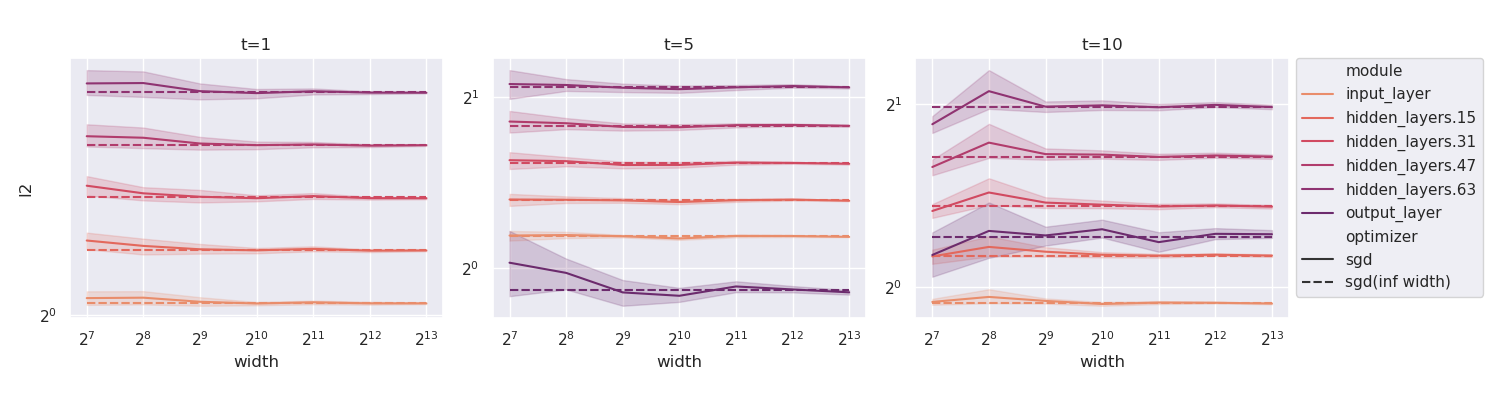
\includegraphics[width=\textwidth]{fig/linear_finite_verify_d64_1510.png}
    \caption{Trained linear network  converges to its infinite width limit which is computed recursively based on $\Gamma$ and $C$. Depth is fixed at 64,width varies between $2^7, 2^8, \ldots, 2^{13}$. Networks are trained with SGD for 10 steps. The root mean square statistics ($y$-axis) at 1st, 5th and 10th steps are plotted using solid lines where the $x$-axis is the width. The root mean square values are computed on the outputs of some of the layers (including the input layer, output layer, and hidden layers at each quarter). The corresponding value for the infinite width is indicated with dashed lines.  }
    \label{fig:verify-linear-finite-d64}
\end{figure}

\begin{figure}
    \centering
    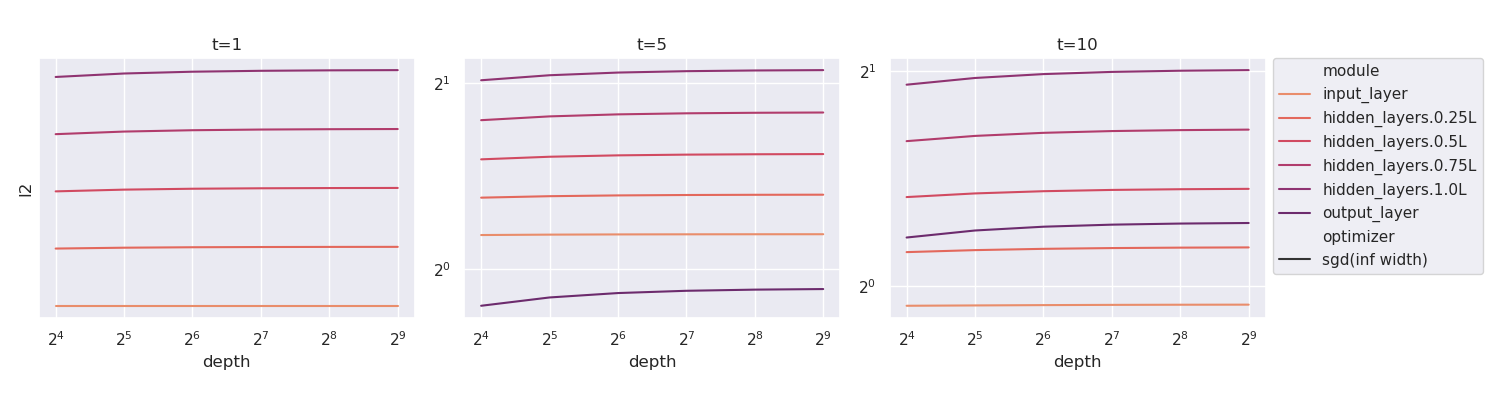
\includegraphics[width=\textwidth]{fig/linear_infinite_verify_1510.png}
    \caption{Under Depth-$\mu$P, infinite wide linear network training converges when increasing the depth. Infinite wide linear networks of depth $2^4, 2^5, \ldots, 2^{9}$  are computed recursively based on $\Gamma$ and $C$. The root mean square statistics ($y$-axis) at 1st, 5th and 10th steps are plotted across the depth ($x$-axis). }
    \label{fig:verify-linear-infinite}
\end{figure}

\section{Experiments}\label{sec:exp}

\subsection{Verifying the Theory in the Linear Case}\label{sec:verify_linear}

In \Cref{sec:linearsgd}, we showed that a complete description of the training dynamics of linear networks can be formulated in terms of  $\Gamma$ and $C$. In this section, we provide empirical results supporting our theoretical findings. We first verify the finite-depth recursive formula for $\Gamma$ in \Cref{lemma:finite_depth_gamma} is the correct limit when the width goes to infinity, then proceed to show that the infinite-depth limit is the correct one.

\paragraph{Infinite-width limit.} In \Cref{fig:verify-linear-finite-d64}, we train a series of $64$-layer linear networks of width $2^7, 2^8, \ldots, 2^{13}$ with $1, 5, 10$ steps on MNIST, and plot the root mean square\footnote{The root mean square of a vector $x=(x_1,\ldots, x_n)$ is $\sqrt{\frac{\sum_{i=1}^n x_i^2}{n}}$, which is denoted as ``l2'' in \Cref{fig:verify-linear-finite-d64,fig:verify-linear-infinite}.} of the layer outputs using solid lines. We also compute the infinite width limit of the corresponding statistics using the recursive formula for $\Gamma$ and plot them as dashed horizontal lines. For clarity of the figure, we only plot the statistics of the input layer, output layer, and hidden layers of index 16, 32, 48, and 64. It is clear that as the width grows, the solid lines converge to the dashed lines consistently across the training steps. It indicates that our computation of the infinite width limit is correct.

\paragraph{Infinite-depth limit.} We verify that the infinite \emph{width} limit above converges when the \emph{depth} grows. We consider linear networks of the same architecture but vary the depth from $2^4$ to $2^9$. We again compute the root mean square values of the layer outputs using the recursive formula for $\Gamma$, and plot them in \Cref{fig:verify-linear-infinite} with depth being $x$-axis. For clarity of the figure, we only plot the statistics of the input layer, output layer, and hidden layers of index $L/4$, $L/2$, $3L/4$, and $L$. One can observe that the statistics of the layer outputs converge quickly when the depth grows from $2^4$ to $2^9$, which verifies our convergence result.

    

\begin{figure}[h]
    \centering
    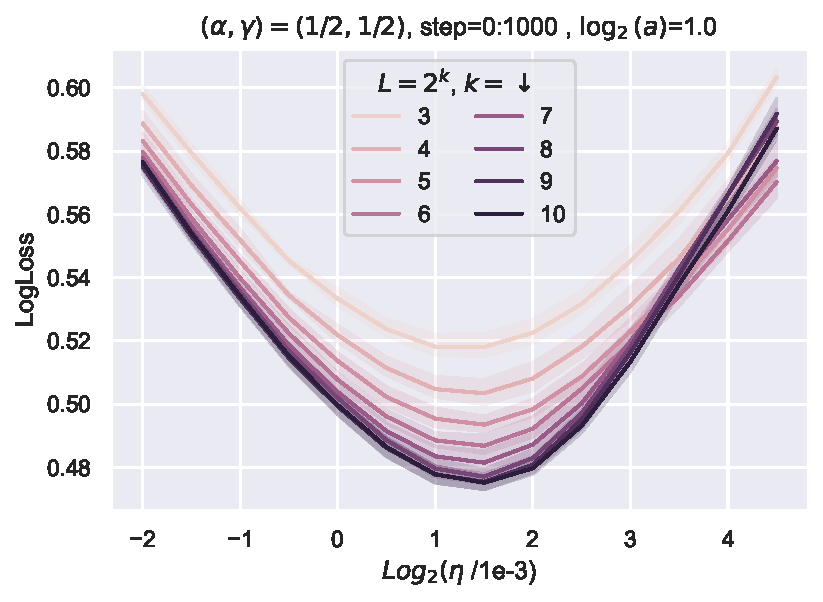
\includegraphics[width=0.45\linewidth]{fig/mup_0.pdf}
    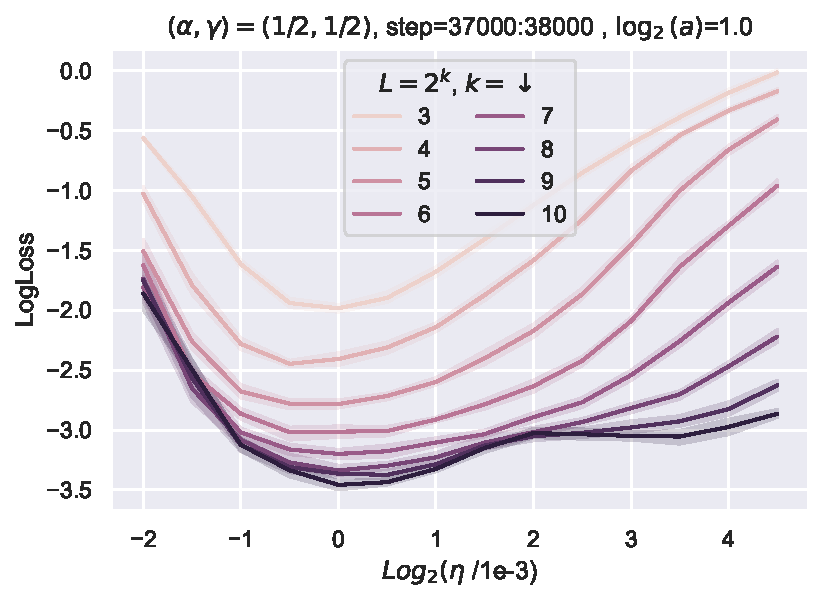
\includegraphics[width=0.45\linewidth]{fig/mup_37000.pdf}

    %
    %

    \centering
    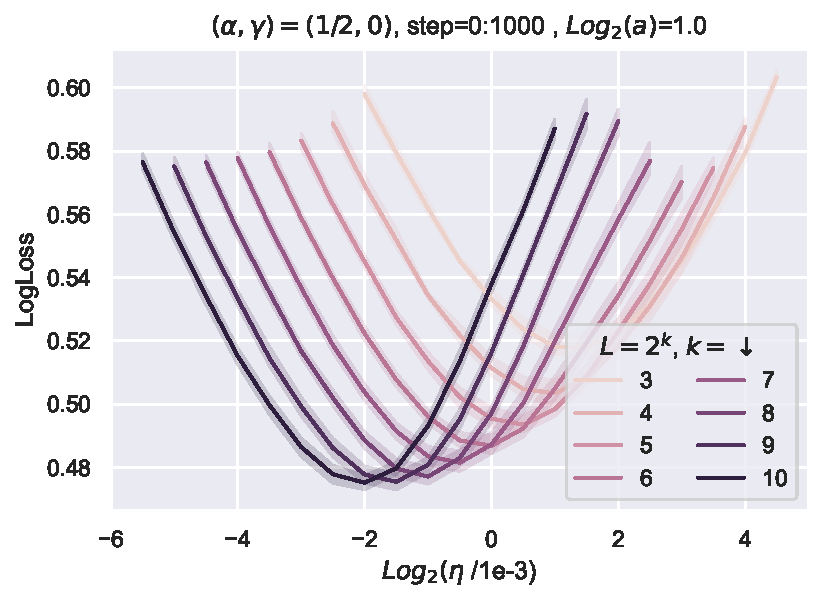
\includegraphics[width=0.45\linewidth]{fig/mup_bl_no_lr_0.pdf}
    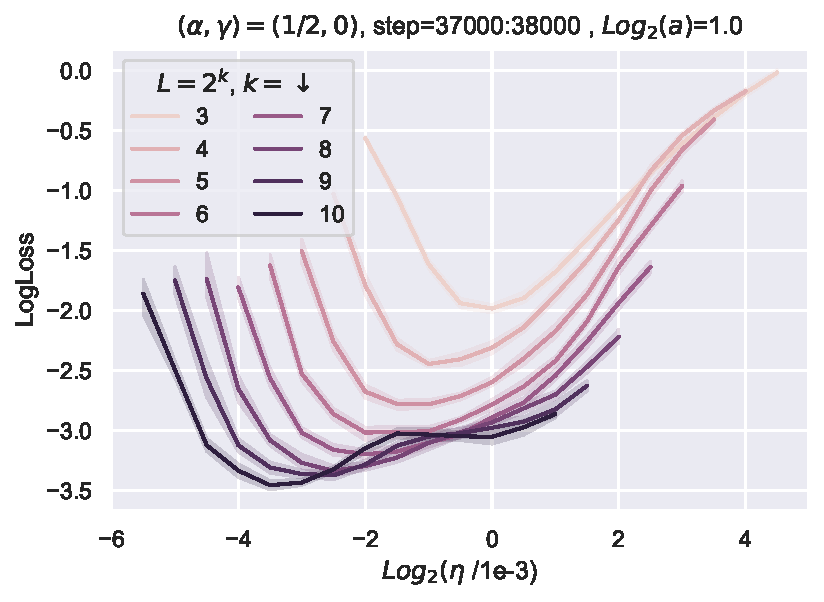
\includegraphics[width=0.45\linewidth]{fig/mup_bl_no_lr_37000.pdf}

    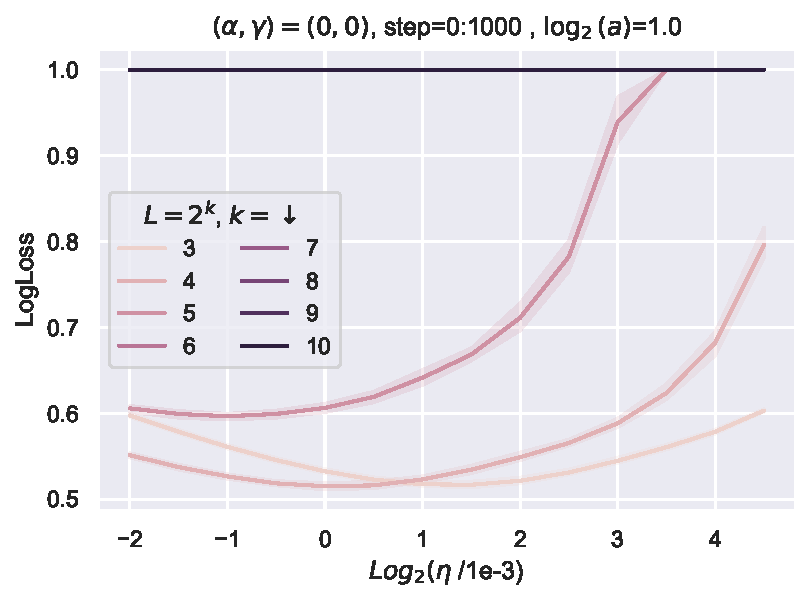
\includegraphics[width=0.45\linewidth]{fig/sp_0.pdf}
    %
    %
        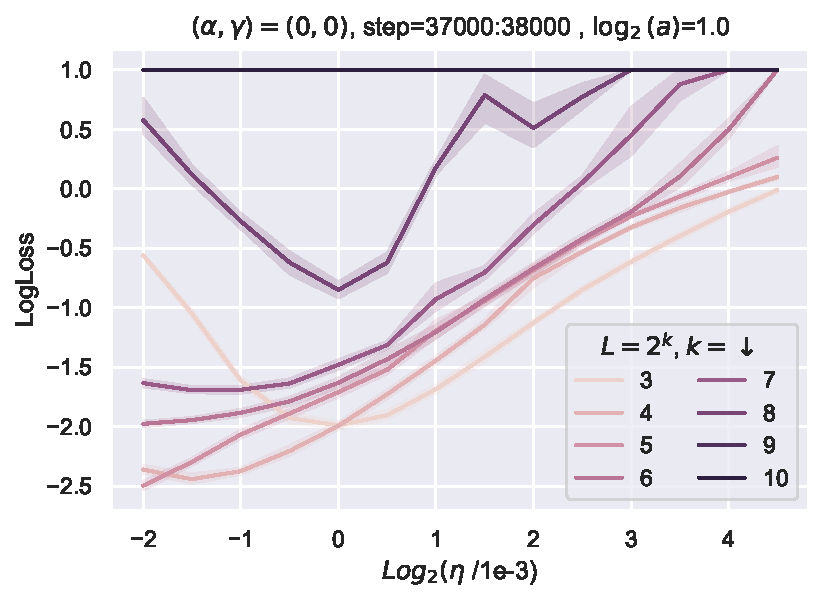
\includegraphics[width=0.45\linewidth]{fig/sp_37000.pdf}
    
    \caption{Train logloss versus learning rate for width $n=256$ and varying depths. The network consists of MLP blocks (with block depth 1), trained for 50 epochs on CIFAR10 dataset using Adam. The batch size is fixed to $64$. We tune the depth $2^3$ network to obtain the optimal $(\log_2(a), \log_2(\eta/1e-3)) = (1, 0)$, and scale all deeper networks using $2^3$ as base depth. The reader can check that the $L=2^3$ curves in each columns are the same. We show the logloss versus the learning rate of the hidden layers (input/output layers fixed) for three parametrizations: Depth-$\mu$P (\textbf{Top}), Scaling only the blocks (no LR scaling), i.e. $\gamma=0$ (\textbf{Middle}), and Standard Parametrization without any scaling ($\alpha=\gamma=0$) (\textbf{Bottom}). Each curve represents the average training loss over a time slice of 1000 steps for depths $2^k$ for $k\in \{1,2,\dots,10\}$. Confidence intervals are based on 5 seeds. The results show that Depth-$\mu$P preserves the optimal learning rate while consistently improving the training loss as depth increases. If we only scale the blocks without scaling the LR ($\alpha=1/2, \gamma=0$) when training with Adam, the optimal learning rate shifts significantly with depth. With standard parametrization without any depth scaling (common practice), the results show a significant shift in the optimal learning rate as well.
    For SP, we cap the log loss at 1, which is why for depth $2^9, 2^{10}$, we have a black horizontal line at $LogLoss=1$.
    %
    }
    \label{fig:lr_transfer}
    \vspace{-0.5cm}
\end{figure}

\subsection{Hyperparameter Transfer}
In this section, we provide empirical evidence to show the optimality of Depth-$\mu$P scaling and the transferability of some quantities across depth. We train vanilla residual network with block depth 1 (1 MLP layer in each residual block) on CIFAR-10 dataset using Adam optimizer, batch size $64$, for $50$ epochs (input and output layers are fixed). The network is parameterized as 
follows
$$
x^l = x^{l-1}+ a \times L^{-\alpha} \textrm{MS}(\phi(W^l x^{l-1})),
$$
and the weights are trained with the rule
$$
  W^{l}\gets W^{l}-\eta \times n^{-1} L^{-\gamma}Q^l_t(n L^{\delta} g_{0},\ldots,n L^{\delta} g_{t}),
$$
where the learning rate $\eta$ and the block multiplier $a$ are the \emph{hyperparameters}.\footnote{Note that $\eta$ here is the constant, and the effective learning rate is given by $\eta n^{-1} L^{-\gamma}$.} The values of $\alpha, \gamma$ depend on the parametrization of choice. For Depth-$\mu$P, we have $\alpha=\gamma=1/2$, and for standard parametrization, we have $\alpha=0,\gamma=1$.\footnote{In standard parametrization, there is generally no rule to scale the learning rate with depth, and the optimal learning rate is typically found by grid search. Here, we assume that in standard parametrization, the learning rate is scaled by $L^{-1}$ to preserve faithfulness.} In our experiments, we assume base depth $8$, meaning that we replace $L$ by $L/8$ in the parametrization above.

\paragraph{Learning rate transfer ($\eta$). }In \Cref{fig:lr_transfer}, we show the training loss versus learning rate for depths $2^k$, for $k\in \{3,4\dots,10\}$. For Depth-$\mu$P, a convergence pattern can be observed for the optimal learning rate as depth grows. Optimal learning rates for small depths (e.g. $L=2^3$) exhibit a mild shift which should be expected, as our theory shows convergence in the large depth limit.  However, starting from depth $L=2^6$, the optimal learning rate is concentrated around $10^{-3}$. 
For parametrization that only scales the multiplier but not LR ($\alpha=1/2$, $\gamma=0$), we observe the optimal learning rate shifts significantly. 
For standard parametrization without any depth scaling  ($\alpha=\gamma=0$), the optimal learning rate exhibits a more significant shift as depth grows. Moreover, even if one picks the optimal learning rate for each depth, the performance still degrades when the depth is very large, suggesting that standard parametrization is not suitable for depth scaling. Additional figures with multiple time slices are provided in \Cref{sec:additional_exps}.

\paragraph{Is feature learning sufficient for HP transfer?} In \Cref{sec:cause_hp}, we explained when and why hyperparameter transfer occurs. Precisely, to obtain HP transfer, one needs to classify all feature learning limits and choose the optimal one. We introduced the notion of feature diversity and showed that Depth-$\mu$P is optimal in the sense that it maximizes feature diversity. To show that optimality is needed for HP transfer, we train a resnet with $(\alpha, \gamma)=(1,0)$ which is also a feature learning limit. \Cref{fig:ode_limit} shows that in this case the learning rate exhibits a significant shift with depth. Interestingly, the constant $\eta$ in this case seems to increase with depth, suggesting that the network is trying to break from the \emph{ODE} limit, which is sub-optimal. Note that in \Cref{fig:lr_transfer}, with Depth-$\mu$P we obtain better training loss compared to the ODE parametrization in \Cref{fig:ode_limit}.

\begin{figure}[h]
    \centering
    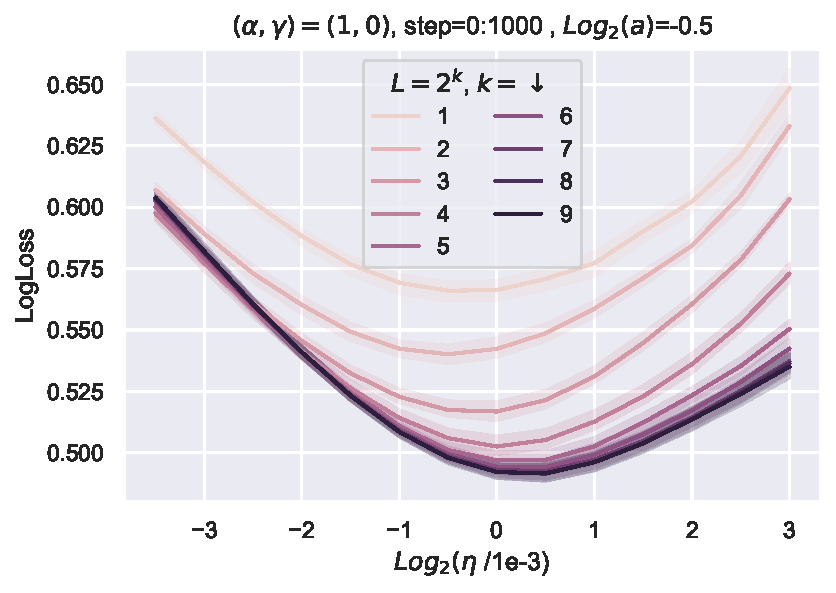
\includegraphics[width=0.45\linewidth]{fig/ode_0.pdf}
    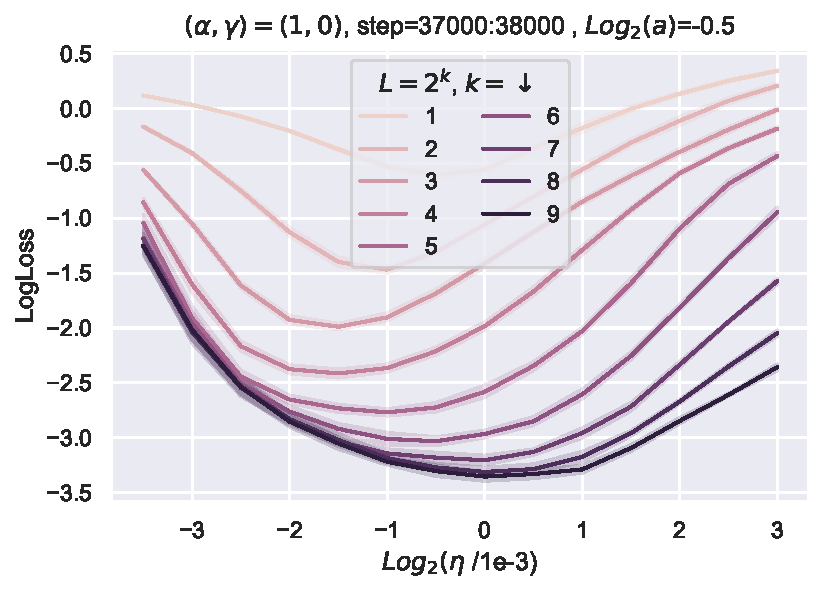
\includegraphics[width=0.45\linewidth]{fig/ode_37000.pdf}
    \caption{Same setup as \cref{fig:lr_transfer} for the parametrization $(\alpha,\gamma)=(1,0)$ (the ODE limit).}
    \label{fig:ode_limit}
\end{figure}

\paragraph{Do we still have transfer with LayerNorm (LN)?} Our theory considers only Mean Substraction (MS), and \Cref{fig:lr_transfer} shows the results with MS. To see wether LN affects HP transfer, we train resnets with the same setup as \Cref{fig:lr_transfer} with absolute value non-linearity and LN applied to $x^{l-1}$ before matrix multiplication with $W^l$ (preLN). We keep MS after non-linearity although it can be removed since LN is applied in the next layer. Our results, reported in \Cref{fig:lr_transfer_ln} suggest that Depth-$\mu$P guarantees learning rate transfer with LN as well.

\begin{figure}[h]
    \centering
    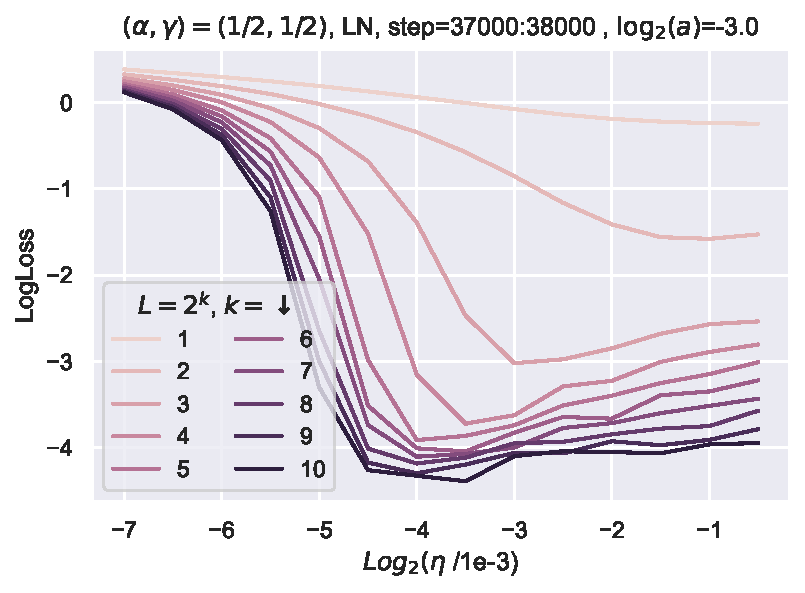
\includegraphics[width=0.45\linewidth]{fig/abs_mup_LN_37000.pdf}
    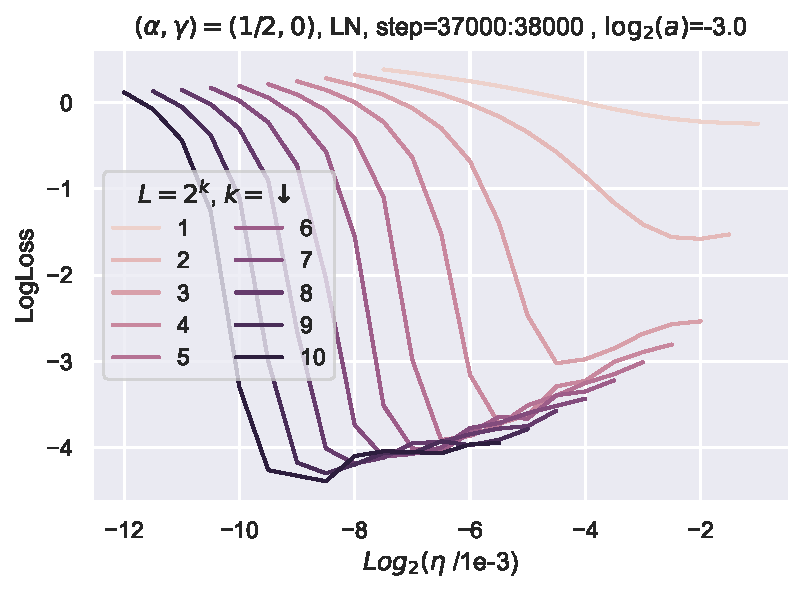
\includegraphics[width=0.45\linewidth]{fig/abs_mup_LN_no_lr_scaling_37000.pdf}

    \caption{Same setup as \Cref{fig:lr_transfer} with Abs non-linearity instead of ReLU and LayerNorm applied to $x^{l-1}$ before matrix multiplication with $W^l$. We show the logloss versus the learning rate of the hidden layers (input/output layers fixed) for two parametrizations: Depth-$\mu$P (\textbf{Left}) and scaling only the blocks without LR scaling ($(\alpha,\gamma)=(1/2,0)$) (\textbf{Right}). The results show that Depth-$\mu$P preserves the optimal learning rate while consistently improving the training loss as depth increases. If we only scale the blocks without scaling the LR ($\alpha=1/2, \gamma=0$) when training with Adam, the optimal learning rate shifts significantly with depth. }
    \label{fig:lr_transfer_ln}
\end{figure}

\paragraph{Block multiplier transfer ($a$).}
In \Cref{fig:blockmult_transfer}, we investigate the stability of the hyperparameter $a$ in Depth-$\mu$P as depth increases. The results suggest that the optimal value of this constant converges as depth grows, which suggest transferability. Additional experiments with multiple time slices are provided in \Cref{sec:additional_exps}.

\begin{figure}[h]
    \centering
    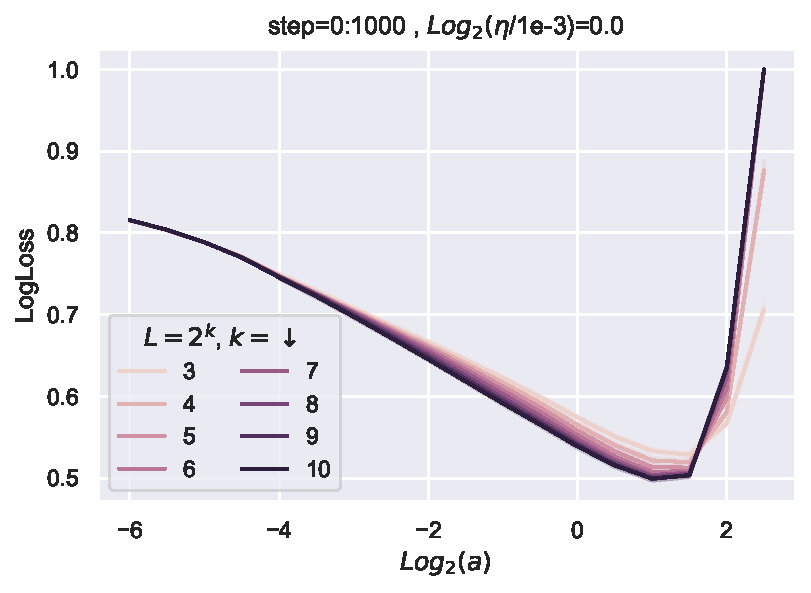
\includegraphics[width=0.45\linewidth]{fig/loss_VS_a_0.pdf}
    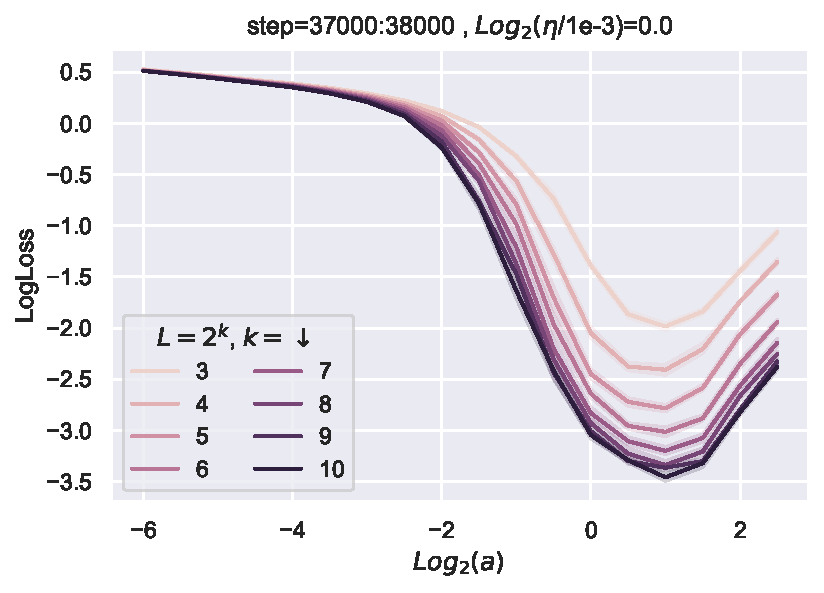
\includegraphics[width=0.45\linewidth]{fig/loss_VS_a_37000.pdf}

    
    \caption{Train logloss versus block multiplier $a$ for varying depths. Same training setup as in \cref{fig:lr_transfer}. The results suggest that Depth-$\mu$P stabilizes the hyperparameter $a$ as depth increases.}
    \label{fig:blockmult_transfer}
\end{figure}

\subsection{What Happens in a Transformer?}

\begin{figure}[h]
    \centering
    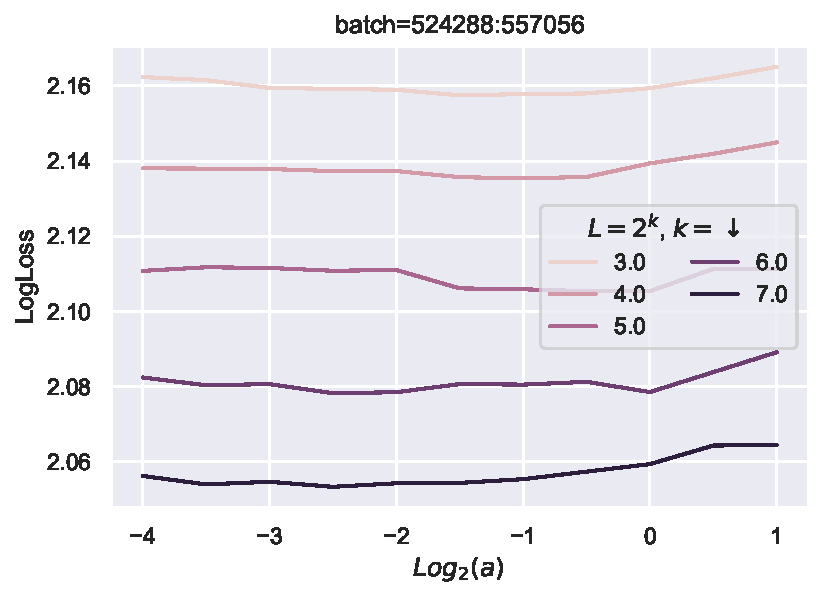
\includegraphics[width=0.45\linewidth]{fig/megatron_bm_insensitive_524288.pdf}
    \caption{Modern transformers are insensitive to block multiplier $a$.}
    \label{fig:megatron_bm_insensitive}
\end{figure}

\begin{figure}[h]
    \centering
    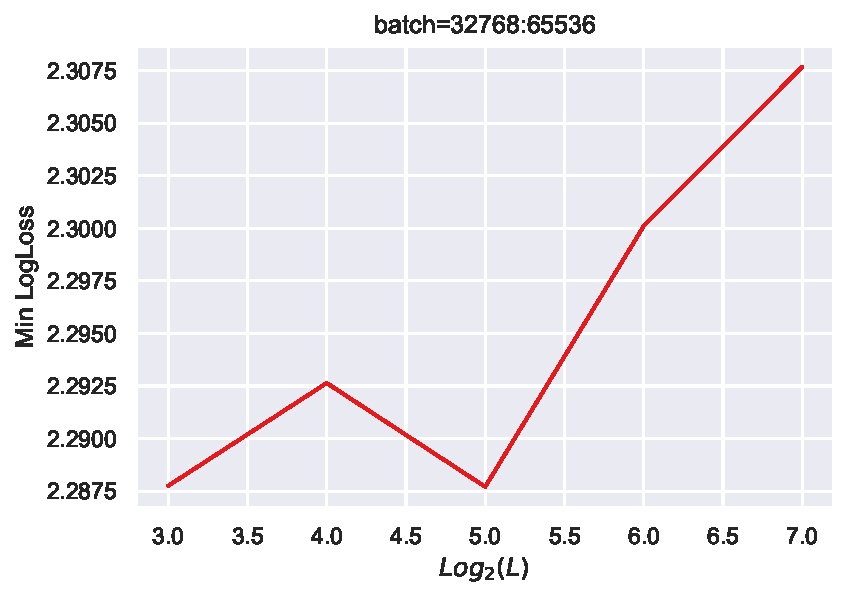
\includegraphics[width=0.4\linewidth]{fig/megatron_minimal_loss_32768.pdf}
    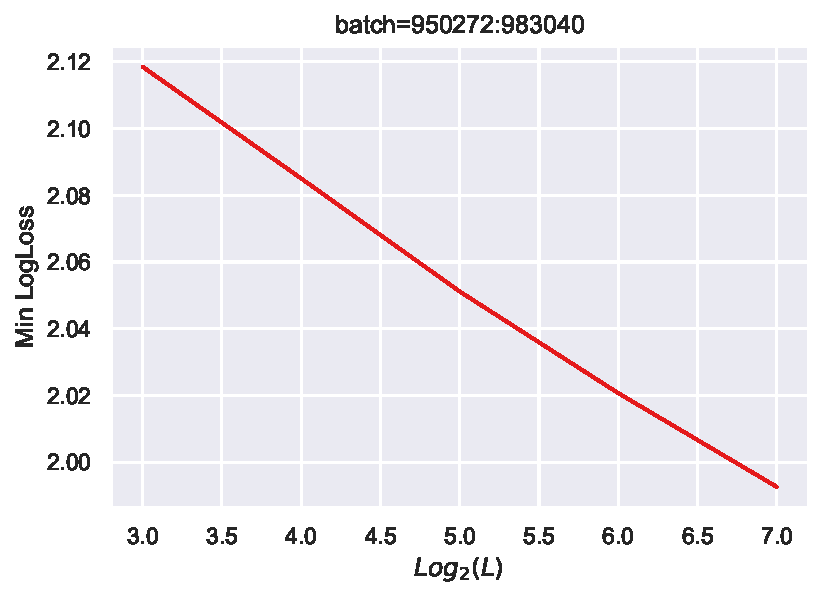
\includegraphics[width=0.4\linewidth]{fig/megatron_minimal_loss_950272.pdf}
    \caption{In (Megatron) Transformer trained on Common Crawl, deeper does worse initially (Left) but eventually does better (Right).}
    \label{fig:megatron-deeper-worse}
\end{figure}

\begin{figure}[h]
    \centering
    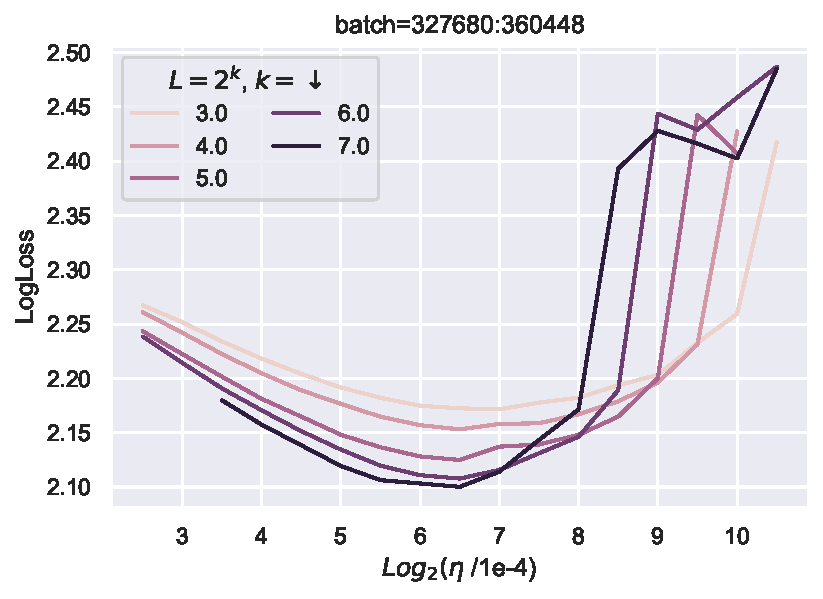
\includegraphics[width=0.4\linewidth]{fig/megatron_1scaling_327680.pdf}
    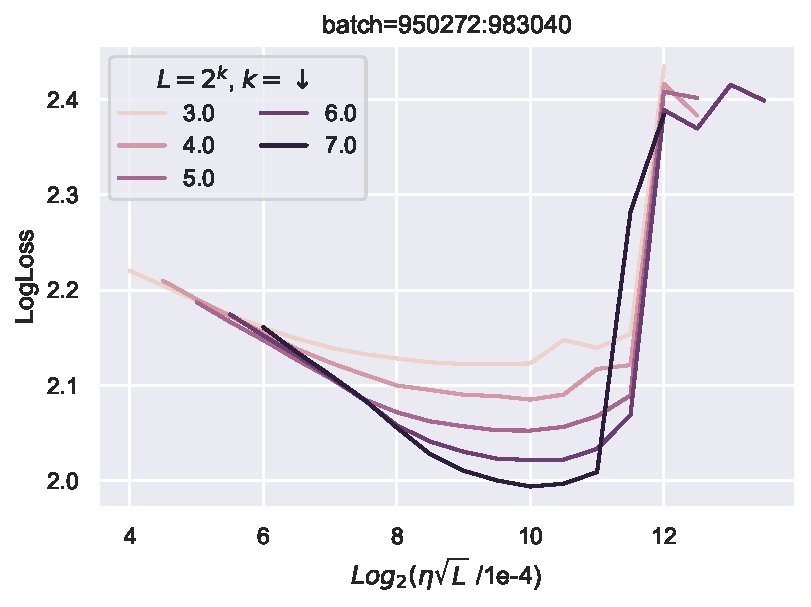
\includegraphics[width=0.4\linewidth]{fig/megatron_sqrt_scaling950272.pdf}
    \caption{In the middle of (Megatron) transformer training, optimal learning rate is approximately invariant (Left), while at the end of training, it approximately scales like $1/\sqrt{L}$. However, the $1/\sqrt{L}$ scaling transfers the maximum viable learning rate better in either case. }
    \label{fig:megatron-scaling-shifts}
\end{figure}

Because transformers have block depth 2, as discussed in \cref{sec:bd2}, we have plenty of reasons to suspect that no parametrization of (learning rate, block multiplier) will be able to robustly transfer hyperparameters across depth for transformers.

Here we do a large scale experiment using Megatron trained on Common Crawl and catalogue our observations.\footnote{We train the models for 3900 steps, using cosine decay schedule with 500 warmup steps. We use a sequence length of 4096, batch size 256, resulting in approximately 4B tokens per training run.}
In summary, in our particular setup (which should be close to most large language model pretraining), we see that the $1/\sqrt L$ scaling seems to transfer hyperparameters at the end of training (\Cref{{fig:megatron-scaling-shifts}}(Right)). However, we also see that 1) deeper does worse in initial training (\Cref{{fig:megatron-deeper-worse}}(Left)), and 2) optimal hyperparameters scale like $\Theta(1)$ in the middle of training (\Cref{fig:megatron-scaling-shifts}(Left)).
Combined with the theoretical insights of \Cref{sec:bd2}, this leads us to conclude that while the $1/\sqrt L$ scaling can potentially be practically useful in transformer training, it is likely to be brittle to architectural  and algorithmic changes, or even simple things like training time.

In fact, we observe that transformers are insensitive to the block multiplier $a$ (\Cref{fig:megatron_bm_insensitive}), so that the only relevant hyperparameter is really just learning rate. Thus, empirically measuring the scaling trend of the optimal learning rate, as done in modern large scale pretraining, can be a practically more robust way to transfer hyperparameters.

Here $L$ is the number of transformer layers, each of which consists of an attention layer and an MLP layer (each of which has depth 2).

\subsection{Feature Diversity}

In this section, we empirically verify our claims about feature diversity exponent (\Cref{clm:redundant,clm:depth_mup}). We use the same setup as in the last section, i.e., we train deep residual networks of width $n=256$ on CIFAR-10 dataset with Adam and batch size $64$. In \Cref{fig:feature-diversity}, we compare two parametrizations, Depth-$\mu$P ($\alpha=\gamma=1/2$) and the ODE parametrization $(\alpha,\gamma)=(1,0)$. We measure $\left\| \xx^{\lfloor (\lambda + \epsilon) L \rfloor}_t - \xx_t^{\lfloor \lambda L \rfloor} \right\|\odefeq d(\epsilon)$ at $t=1000$ for the two parametrizations and varying depth. For each parametrization and depth $L$, we rescale function $d$ by multiplying a constant $c$ such that $c\cdot d(1/256)=1$, and then plot the rescaled function $c\cdot d$ for a clean presentation. One can observe clearly that Depth-$\mu$P has feature diversity exponent (almost) $1/2$ for any $L$, while the curves for ODE parametrization move from $\epsilon^{1/2}$ to $\epsilon$ when $L$ grows.   This exactly fits our theory that Depth-$\mu$P maximizes the feature diversity, while other parametrizations (even with feature learning) have smaller feature diversity exponents that should go to $0$ in the infinite depth limit.

\paragraph{Growth along with $L$ and $t$.} In \Cref{fig:feature-diversity-ode}, we measure $d(\epsilon)$ at $t=100, 500, 1000$, and rescale it by \emph{dividing} \emph{additional} $\epsilon^{0.5}$ and a constant $c$ such that $\frac{d(1/256)}{c\cdot \epsilon^{0.5}}=1$, and then plot the rescaled function $d/(c\cdot \epsilon^{0.5})$ for a clean comparison between $d$ and $\epsilon^{0.5}$. We observe that for both Depth-$\mu$P and ODE parametrization, the slopes of the curves grow along with $L$ and $t$. The growth along $t$ can be explained by the cumulative correlation between layers. The growth along $L$ for ODE parametrization is because the independent components between nearby layers decrease when $L$ grows. We do not have a clear understanding for the growth along $L$ for Depth-$\mu$P and we leave it as a future work.

\paragraph{Absolute value activation increases feature diversity.} In \Cref{fig:feature-diversity-abs}, we plot the same curves as in \Cref{fig:feature-diversity-ode} but comparing ReLU activation and absolute value activation under Depth-$\mu$P. We observe that the slope of the curves for absolute value activation is smaller than ReLU activation. It matches our theory that absolute value activation increases feature diversity.

\begin{figure}[t]
    \centering
    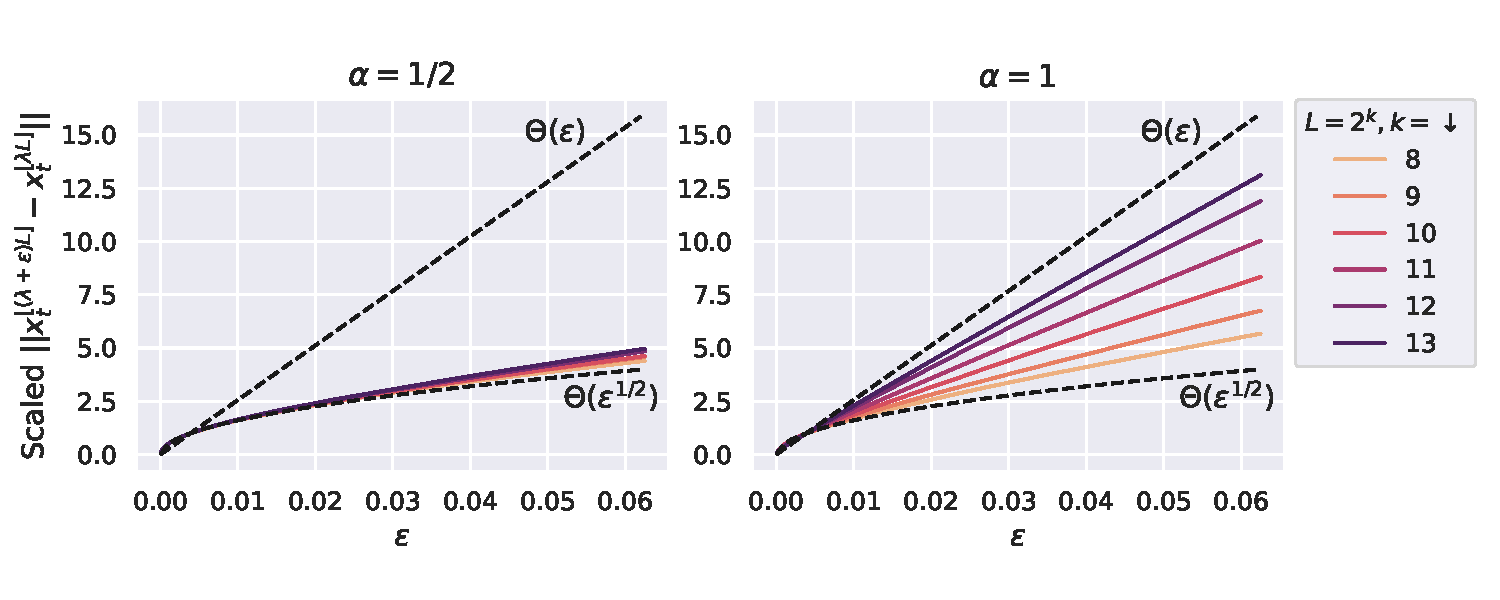
\includegraphics[width=\textwidth]{fig/feature_diversity.pdf}
    \caption{Difference between feature at layer $\lfloor\lambda L\rfloor$ and feature at layer $\lfloor(\lambda+\epsilon)L\rfloor$ as a curve of $\epsilon$ for width $n=256$ and varying depths. For a clean presentation, each curve is scaled by a constant so it always passes $(1/256, 1)$. The feature diversity exponent $\kappa$ depends on the growth of the curve when $L\to\infty$. For Depth-$\mu$P (left), the curve is always close to $\epsilon^{1/2}$, meaning $\kappa=1/2$. For ODE parametrization (right), the curve shifts from $\epsilon^{1/2}$ to $\epsilon$ when $L$ grows, indicating its $\kappa$ goes to $0$ in the infinite depth limit. }
    \label{fig:feature-diversity}
\end{figure}

\begin{figure}[t]
    \centering
    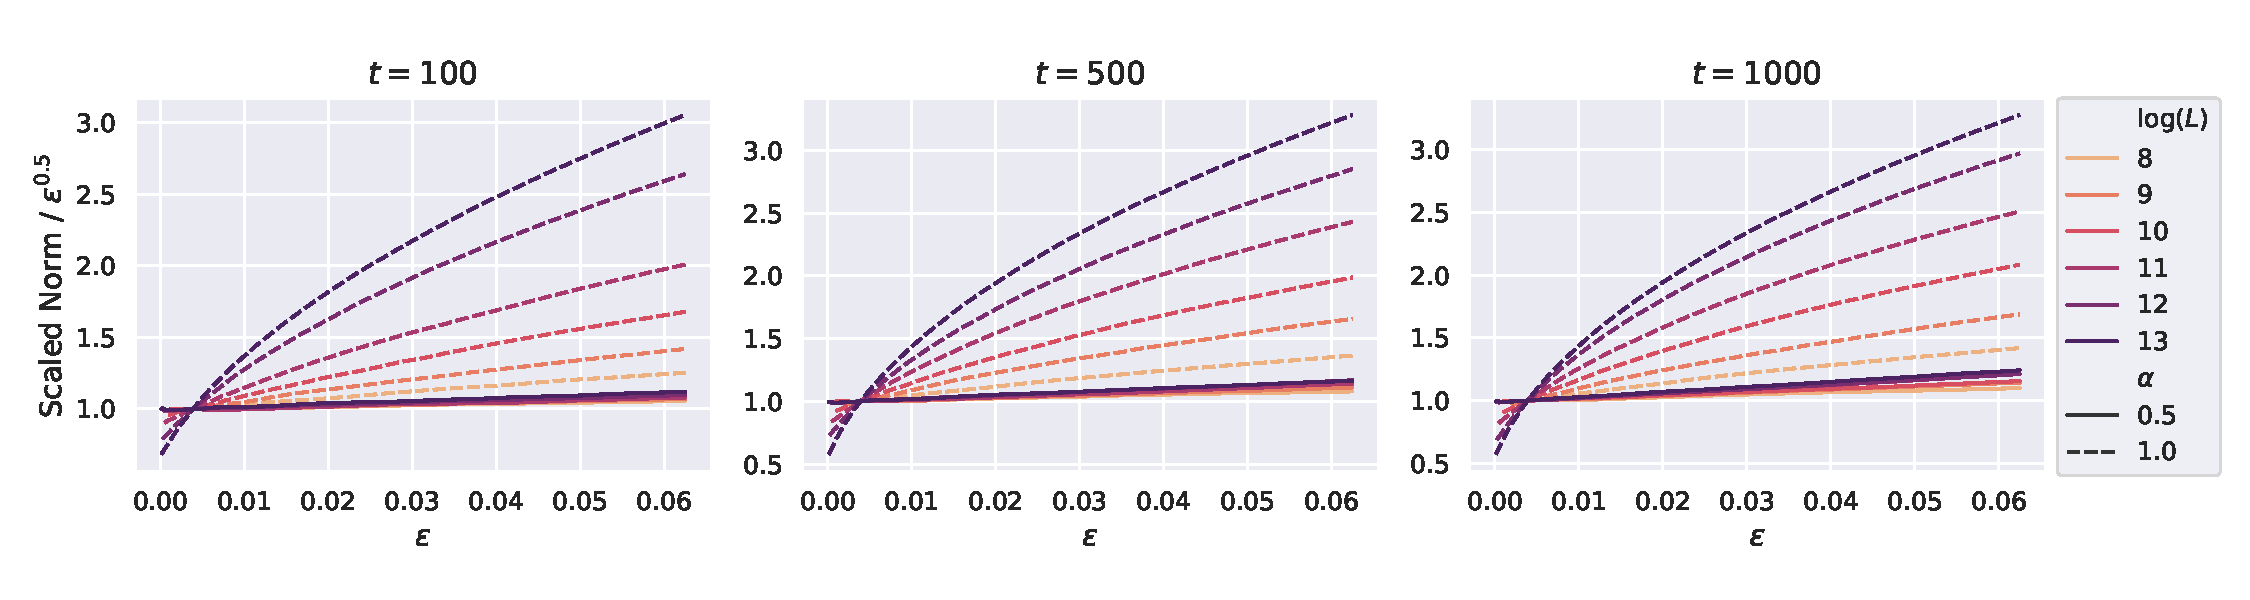
\includegraphics[width=\textwidth]{fig/feature_diversity_ode.pdf}
    \caption{Same setup as \Cref{fig:feature-diversity} but at step $t=100, 500, 1000$, and each curve is scaled by dividing a constant and \emph{additional} $\epsilon^{1/2}$ so it always passes $(1/256, 1)$. The curve indicating feature diversity exponent $\kappa$ exactly $1/2$ should be a horizontal line at $1$. For Depth-$\mu$P ($\alpha=0.5$), the curves are almost horizontal. For ODE parametrization ($\alpha=1$), slopes of the curves are larger with larger $L$ and larger $t$.}
    \label{fig:feature-diversity-ode}
\end{figure}

\begin{figure}[t]
    \centering
    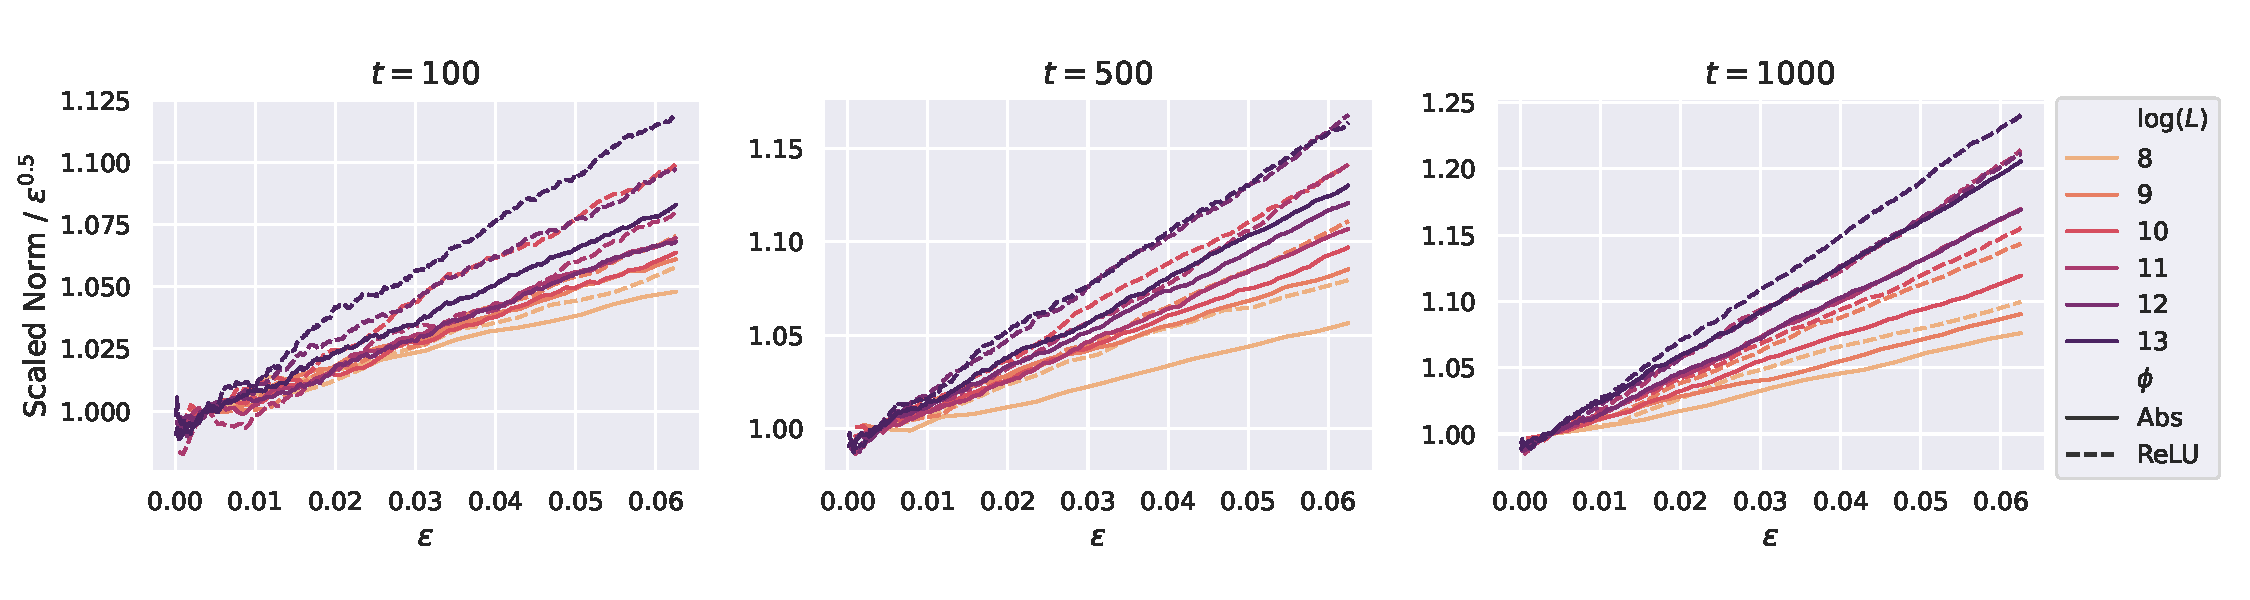
\includegraphics[width=\textwidth]{fig/feature_diversity_abs.pdf}
    \caption{Same setup as \Cref{fig:feature-diversity-ode}, but comparing Depth-$\mu$P with ReLU activation and absolute value activation. Each curve is scaled by dividing a constant and $\epsilon^{1/2}$ so it always passes $(1/256, 1)$. The curve indicating feature diversity exponent $\kappa$ exactly $1/2$ should be a horizontal line at $1$. For both activations, slopes of curves are small, but growing along with $L$ and $t$. The slopes with absolute value activation 
    ($\phi=\mathrm{Abs}$) are slower than the slopes with ReLU activation ($\phi=\mathrm{ReLU}$), indicating feature diversity is higher with absolute value activation.}
    \label{fig:feature-diversity-abs}
\end{figure}

